\chapter{Registration}

\section{Why?}
\begin{itemize}
\item Image registration \cite{Oliveira25012014} is a digital image
  processing technique that helps us align different images (for
  example, \gls{CT} and \gls{MRI} of the same scene.
\item For example, the registered images can be averaged to increase
  the \gls{SNR}.
\end{itemize}

\begin{figure}[H]
  \vspace{-0ex}
  \centering
  \begin{tabular}{ccc}
    \href{https://d2rfm59k9u0hrr.cloudfront.net/medpix/img/full/synpic50411.jpg}{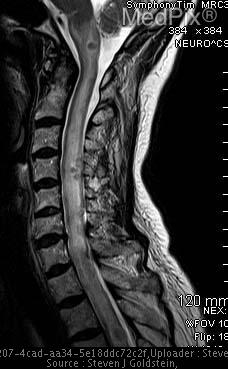
\includegraphics[width=0.25\textwidth]{a1}} & \href{https://d2rfm59k9u0hrr.cloudfront.net/medpix/img/full/synpic50412.jpg}{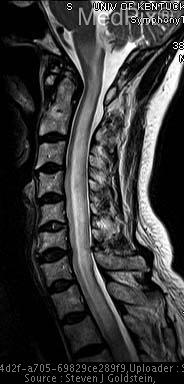
\includegraphics[width=0.25\textwidth]{a2}} & \href{sec:ImageJ_registration}{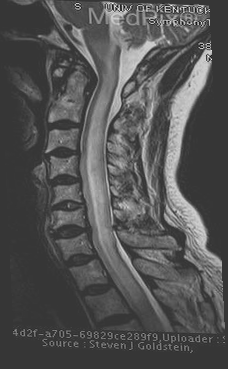
\includegraphics[width=0.25\textwidth]{a3}} \\
    Reference & To warp & Projection
  \end{tabular}
  \caption[Image registration example.]{Image registration
    example. Images source:
    \url{https://medpix.nlm.nih.gov/case?id=414ff6ec-e857-40da-ac84-d3dba505a08a}.}
  \label{fig:image_registration}
\end{figure}
%https://medpix.nlm.nih.gov/case?id=d9f68ce4-ee14-49ea-a50a-19e70dabd239
%https://medpix.nlm.nih.gov/case?id=414ff6ec-e857-40da-ac84-d3dba505a08a

\section{Registration with ImageJ}
\label{sec:ImageJ_registration}
\begin{itemize}
  \item ImageJ
    \cite{abramoff2004image}\footnote{\url{https://imagej.net/ij}} is
    an open-source, Java-based software for processing and analyzing
    2D and 3D scientific images.
\begin{figure}[H]
  \vspace{-0ex}
  \centering
  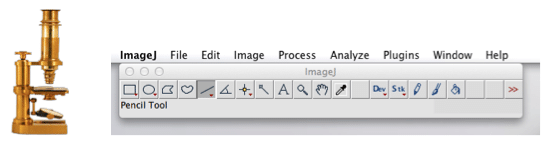
\includegraphics[width=0.75\textwidth]{ImageJ}
  \caption{ImageJ icon and main window.}
  \label{fig:ImageJ}
\end{figure}
  \item To register 2 images there are
    \href{https://imagej.net/imaging/registration}{several}
    \popup{plugins}{A source code Java extension which incorporate
      extra functionality to the basic program}.
\end{itemize}

\begin{itemize}
\item To install a plugin\footnote{\url{https://imagej.net/plugins}} do:
  \begin{enumerate}
  \item Go to the plugins Web page: \url{https://imagej.net/plugins}.
  \item Click in \href{https://imagej.net/list-of-extensions}{List of Extensions}: \url{https://imagej.net/list-of-extensions}.
  \item Search for TurboReg: \url{https://imagej.net/plugins/turboreg}.
  \item Follow the link to the BIG website: \url{https://bigwww.epfl.ch/thevenaz/turboreg/}.
  \item Download the .zip file: \url{http://bigwww.epfl.ch/thevenaz/turboreg/turboreg.zip}.
  \item Unzip it.
  \item Open ImageJ.
  \item Go to \texttt{Plugins} $\rightarrow$ \texttt{Install ...}.
  \item Select the file \texttt{TurboReg\_.jar}.
  \end{enumerate}
  \newpage
\item To use the TurboReg plugin:
  \begin{enumerate}
  \item Load the reference image. For example, \href{https://d2rfm59k9u0hrr.cloudfront.net/medpix/img/full/synpic50411.jpg}{this image}.
  \item Load the image to register. For example, \href{https://d2rfm59k9u0hrr.cloudfront.net/medpix/img/full/synpic50412.jpg}{this image}.
  \item Go to \texttt{Pugins} $\rightarrow$ \texttt{TurboReg}.
  \item Configure and run it.
  \item Save the image, if you are happy with it: \texttt{File}
    $\rightarrow$ \texttt{Save As} $\rightarrow$ (chose the output file
    format).
  \end{enumerate}
\end{itemize}

\begin{comment}
# https://www.geeksforgeeks.org/python/image-registration-using-opencv-python/

import cv2
import numpy as np

# Open the image files.
img1_color = cv2.imread("align.jpg")  # Image to be aligned.
img2_color = cv2.imread("ref.jpg")    # Reference image.

# Convert to grayscale.
img1 = cv2.cvtColor(img1_color, cv2.COLOR_BGR2GRAY)
img2 = cv2.cvtColor(img2_color, cv2.COLOR_BGR2GRAY)
height, width = img2.shape

# Create ORB detector with 5000 features.
orb_detector = cv2.ORB_create(5000)

# Find keypoints and descriptors.
# The first arg is the image, second arg is the mask
#  (which is not required in this case).
kp1, d1 = orb_detector.detectAndCompute(img1, None)
kp2, d2 = orb_detector.detectAndCompute(img2, None)

# Match features between the two images.
# We create a Brute Force matcher with 
# Hamming distance as measurement mode.
matcher = cv2.BFMatcher(cv2.NORM_HAMMING, crossCheck = True)

# Match the two sets of descriptors.
matches = matcher.match(d1, d2)

# Sort matches on the basis of their Hamming distance.
matches.sort(key = lambda x: x.distance)

# Take the top 90 % matches forward.
matches = matches[:int(len(matches)*0.9)]
no_of_matches = len(matches)

# Define empty matrices of shape no_of_matches * 2.
p1 = np.zeros((no_of_matches, 2))
p2 = np.zeros((no_of_matches, 2))

for i in range(len(matches)):
  p1[i, :] = kp1[matches[i].queryIdx].pt
  p2[i, :] = kp2[matches[i].trainIdx].pt

# Find the homography matrix.
homography, mask = cv2.findHomography(p1, p2, cv2.RANSAC)

# Use this matrix to transform the
# colored image wrt the reference image.
transformed_img = cv2.warpPerspective(img1_color,
                    homography, (width, height))

# Save the output.
cv2.imwrite('output.jpg', transformed_img)

\end{comment}

